\documentclass{TIJMUjiaoanSY}
\pagestyle{empty}


\begin{document}


%课程名称
\kecheng{Linux系统概论}
%实验名称
\shiyan{实验8\ shell脚本编程}
%教师姓名
\jiaoshi{伊现富}
%职称
\zhicheng{讲师}
%教学日期(格式:XXXX年XX月XX日XX时-XX时)
\riqi{2015年7月2日15:30-17:30}
%授课对象(格式:XXX系XXXX年级XX班(硕/本/专科))
\duixiang{生物医学工程学院2013级生信班(本)}
%实验人数
\renshu{28}
%实验类型
\leixing{验证型}
%实验分组
\fenzu{一人一机}
%学时数
\xueshi{2}
%教材版本
\jiaocai{Linux系统概论上机指南(自编教材)}


%教案首页
\firstHeader
\maketitle
\thispagestyle{empty}

\mudi{
\begin{itemize}
  \item 掌握shell脚本的结构和运行方法。
  \item 掌握shell函数的使用方法。
  \item 掌握shell脚本中的流程控制。
  \item 掌握shell脚本的调试方法。
\end{itemize}
}

\fenpei{
\begin{itemize}
  \item (5')编程起步:回顾shell脚本的基本结构和运行方法,总结调试shell脚本的主要方法。
  \item (10')流程控制:回顾if-then、case和while、until、for等条件流程控制和迭代流程控制的基本语法。
  \item (5')shell函数:回顾声明和调用shell函数的基本语法,总结嵌套和递归、作用域等相关知识点。
  \item (80')实验操作:练习shell脚本的编写,掌握shell脚本的基本使用。
\end{itemize}
}

\cailiao{
\begin{itemize}
  \item 主要仪器:一台安装有CentOS计算机。
\end{itemize}
}

\zhongdian{
\begin{itemize}
  \item 重点难点:shell中的流程控制语法,shell函数的使用。
  \item 解决策略:通过实例进行讲解,通过演示进行学习,通过练习熟练掌握。
\end{itemize}
}

\sikao{
\begin{itemize}
  \item 如何给变量赋值、访问变量的值?
  \item 总结各种条件流程控制和迭代流程控制的语法结构。
  \item 列举常见的文件测试并解释其含义。
  \item 字符串和整数值比较的运算符有哪些?
  \item 如何声明并调用shell函数?
  \item 如何对shell脚本进行调试?
\end{itemize}
}

\cankao{
\begin{itemize}
  \item Linux基础及应用习题解析与实验指导(第二版),谢蓉\ 编著。中国铁道出版社,2014。
\end{itemize}
}

\firstTail


%教案续页
\newpage
\otherHeader

\noindent
\begin{enumerate}
  \item 编程起步(5分钟)
    \begin{enumerate}
      \item 脚本结构与运行方法
	\vspace*{-10pt}
	\begin{multicols}{2}
	\begin{enumerate}
	  \item 脚本结构
	    \begin{itemize}
	      \item \#!(shebang结构)调用shell
	      \item \#进行注释
	      \item 命令和控制结构
	    \end{itemize}
	  \item 运行方法
	    \begin{itemize}
	      \item 创建文件:vim script.sh
	      \item 修改权限:chmod u+x script.sh
	      \item 运行脚本:./script.sh,sh script.sh
	    \end{itemize}
	\end{enumerate}
	\end{multicols}
	\vspace*{-10pt}
      \item 变量使用
	\begin{itemize}
	  \item 赋值:使用=(赋值运算符),=两边不能有空格,在=后面跟一个换行符赋空值
	  \item 访问:默认情况下将变量视作文本字符串,在变量名前加\$可以访问变量的值 
	  \item 变量名:只能包含字母、数字和下划线,必须以字母或下划线开头,大小写敏感(惯例使用大写)
	\end{itemize}
  \item 脚本调试(5分钟)
    \begin{itemize}
      \item \verb|sh -n script|:检查语法,不执行脚本。
      \item \verb|sh -x script|:执行脚本并显示所有变量的值。
      \item \verb|set -x; command; set +x|:脚本局部调试。
      \item \verb|echo|:打印变量的值、提示信息等来调剂脚本。
    \end{itemize}
    \end{enumerate}

  \item 流程控制(10分钟)
    \begin{enumerate}
      \item 简介
	\begin{itemize}
	  \item 流程控制允许程序做出判断:程序计算条件的值,并根据这些条件执行相应的操作
          \item 条件流程控制:根据特定的约束是否满足来决定是否执行某个代码段
          \item 迭代流程控制:代码块重复或迭代,直到满足某个条件为止
	\end{itemize}
      \item 条件流程控制
	\begin{itemize}
	  \item if-then
	    \begin{itemize}
	      \item if-then
\parpic[fr]{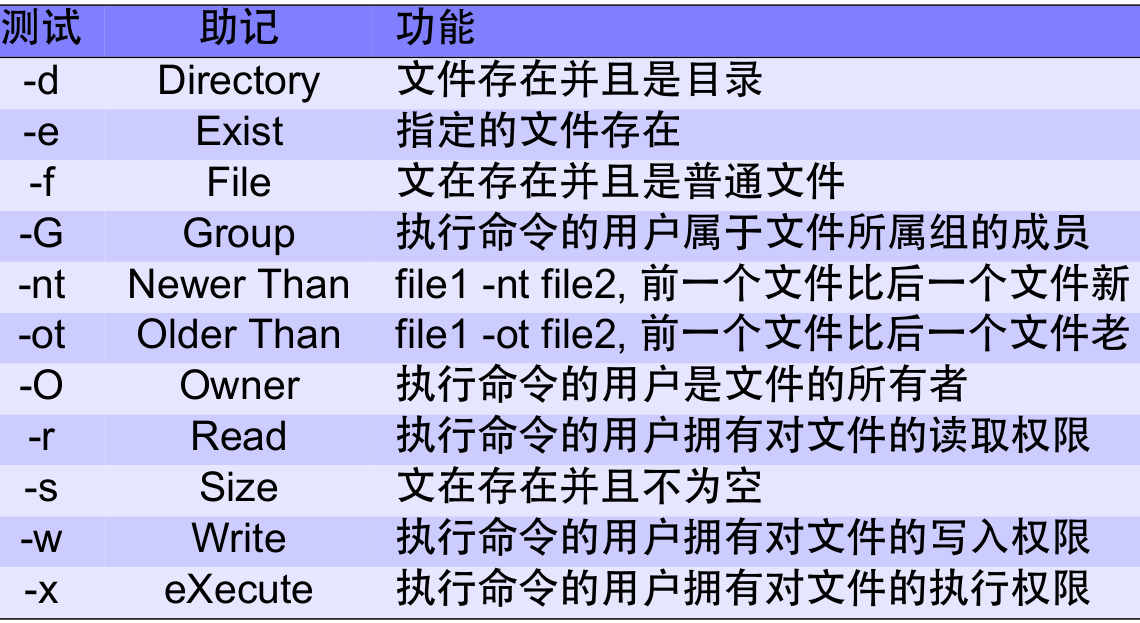
\includegraphics[width=8cm]{c8.test.png}}
\begin{verbatim}
if some_condition
then
  something happens
fi
\end{verbatim}
	      \item if-then-else
\parpic[fr]{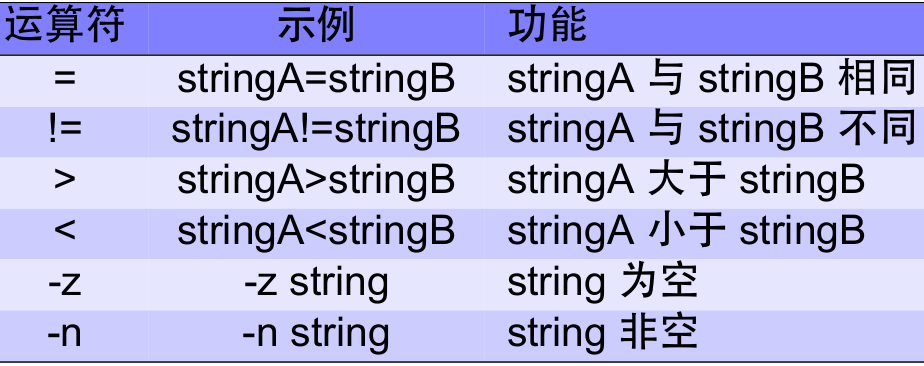
\includegraphics[width=8cm]{c8.compare.01.png}}
\begin{verbatim}
if some_condition
then
  something happens
else
  something happens
fi
\end{verbatim}
	      \item if-then-elif-else
\parpic[fr]{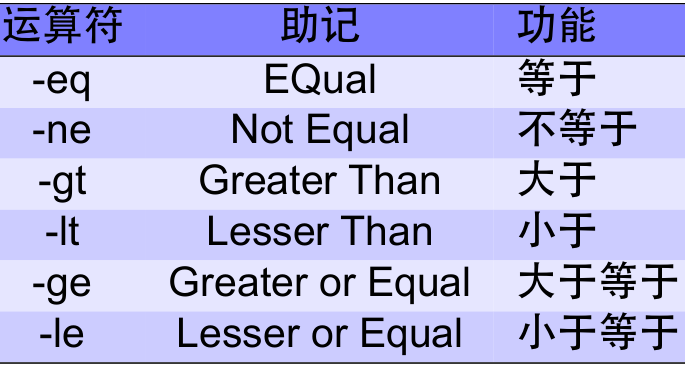
\includegraphics[width=6cm]{c8.compare.02.png}}
\begin{verbatim}
if some_condition
then
  something happens
elif other_condition
  something happens
else
  something happens
fi
\end{verbatim}
	    \end{itemize}
	  \item 比较运算符
	    \begin{itemize}
	      \item 字符串比较
	      \item 整数值比较
	    \end{itemize}

\otherTail
\newpage
\otherHeader

	\vspace*{-10pt}
	\begin{multicols}{2}
	  \item test
	    \begin{itemize}
	      \item 语法
\begin{verbatim}
# 注意中括号内的空格
if [ $COLOR="purple" ]
if (test $COLOR="purple")

# 测试文件是否存在
if [ -e filename ]
if (test -e filename)
\end{verbatim}
	      \item 文件测试
	      \item 逻辑运算符(\verb|&&|、\verb=||=)
	    \end{itemize}
	  \item case
\begin{verbatim}
case expression in
  pattern1)
    action1
    ;;
  pattern2)
    action2
    ;;
  *)
    default action
    ;;
esac
\end{verbatim}
\end{multicols}
	\vspace*{-10pt}

	\end{itemize}

      \item 迭代流程控制
	\vspace*{-10pt}
	\begin{multicols}{3}
	\begin{itemize}
	  \item while
\begin{verbatim}
while condition
do
  action
done
\end{verbatim}

	  \item until
\begin{verbatim}
until condition
do
  action
done
\end{verbatim}
	  \item for
\begin{verbatim}
for VAR in LIST
\end{verbatim}
\begin{verbatim}
do
  action
done
\end{verbatim}
	\end{itemize}
      \end{multicols}
	\vspace*{-10pt}
    \end{enumerate}

  \item shell函数(5分钟)
    \begin{enumerate}
      \item 声明与调用
	\vspace*{-10pt}
	\begin{multicols}{2}
\begin{verbatim}
# 函数声明
name () {
  commands
}
# 函数调用,不带()
name
name parameter(s)
\end{verbatim}
\begin{verbatim}
#!/bin/bash
# A simple function
repeat () {
  echo "I don't know $1 $2"
}
repeat Your Name
# I don't know Your Name
\end{verbatim}
	\end{multicols}
	\vspace*{-10pt}
      \item 嵌套和递归
	\begin{itemize}
	  \item 递归函数:就像调用其他函数一样、调用自己的函数
	  \item 函数嵌套:在一个函数中调用包含在另一个函数中的功能
	\end{itemize}
      \item 作用域
	\begin{itemize}
	  \item 全局作用域:在脚本的任何地方都可以访问变量
	  \item 局部作用域:只能在声明变量的作用域内访问它们
	  \item 使用local关键字定义局部变量
	\end{itemize}
    \end{enumerate}

  \item 实验操作(80分钟)
    \begin{enumerate}
      \item 简单的shell脚本\textcolor{red}{(运行方法)}
      \item shell函数\textcolor{red}{(传递参数,嵌套,作用域)}
      \item shell脚本实例\textcolor{red}{(read,if-then,test,case,for)}
    \end{enumerate}

\end{enumerate}

\otherTail


\end{document}

